\documentclass{article}
% option ``report'' puts title on separate page

\usepackage{amsmath}
\usepackage[pdftex]{graphicx}

\begin{document}

\title{WS3: Numerical Integration}
\author{Jackie Villadsen}
\date{\today}
\maketitle


\section{Integration via Newton-Cotes Formulae}
I compared numerical integration using the Trapezoid Rule and Simpson's
Rule, testing both schemes on two integrals: $\sin(x)$ from 0 to $\pi$,
and $x\sin(x)$ from 0 to $\pi$.

\begin{figure}[h]
  \begin{center}
     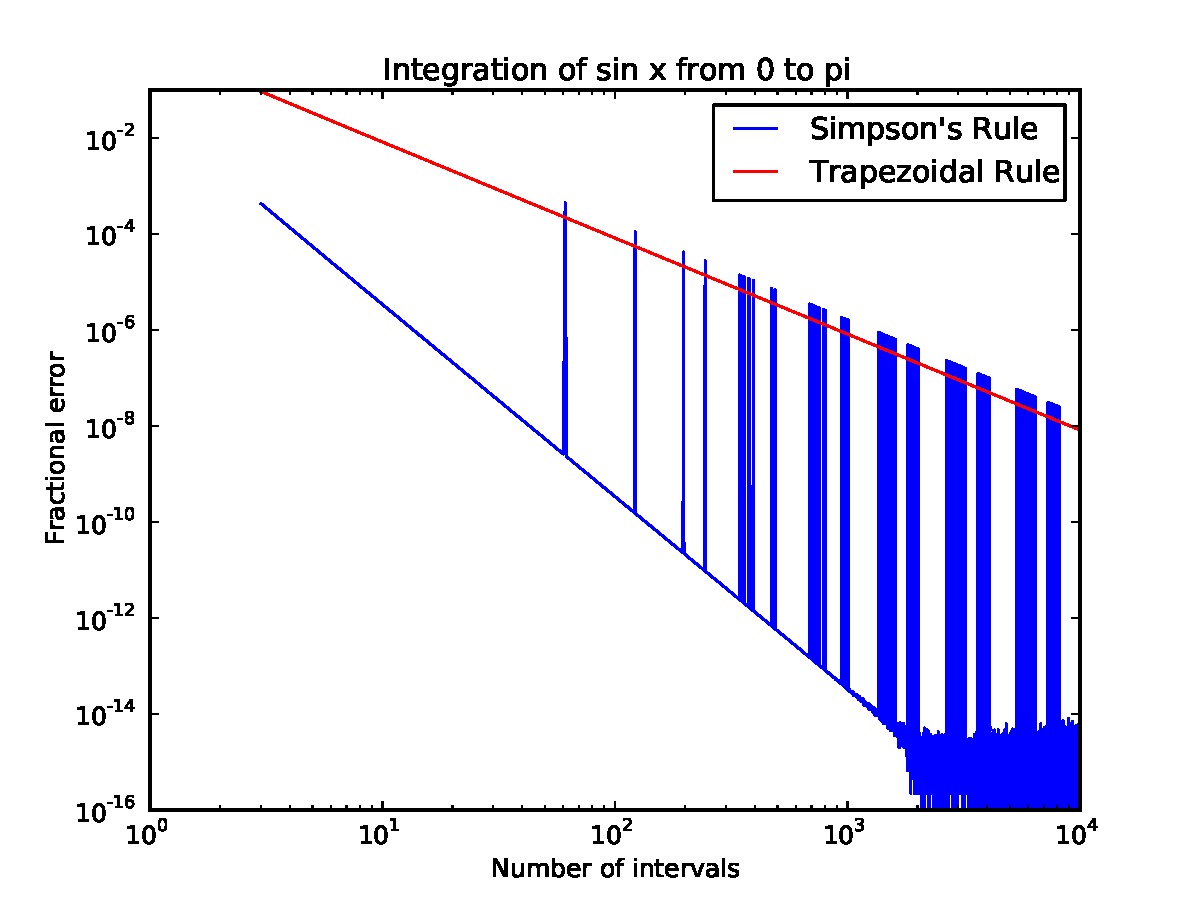
\includegraphics[width=\textwidth]{sinx}
  \end{center}
  \caption{Fractional error on numerical integration of $\sin(x)$ from 0 to $\pi$, using
	   the Trapezoid Rule and Simpson's Rule, for a range of step sizes.}
  \label{fig:sinx}
\end{figure}

\begin{figure}[h]
  \begin{center}
     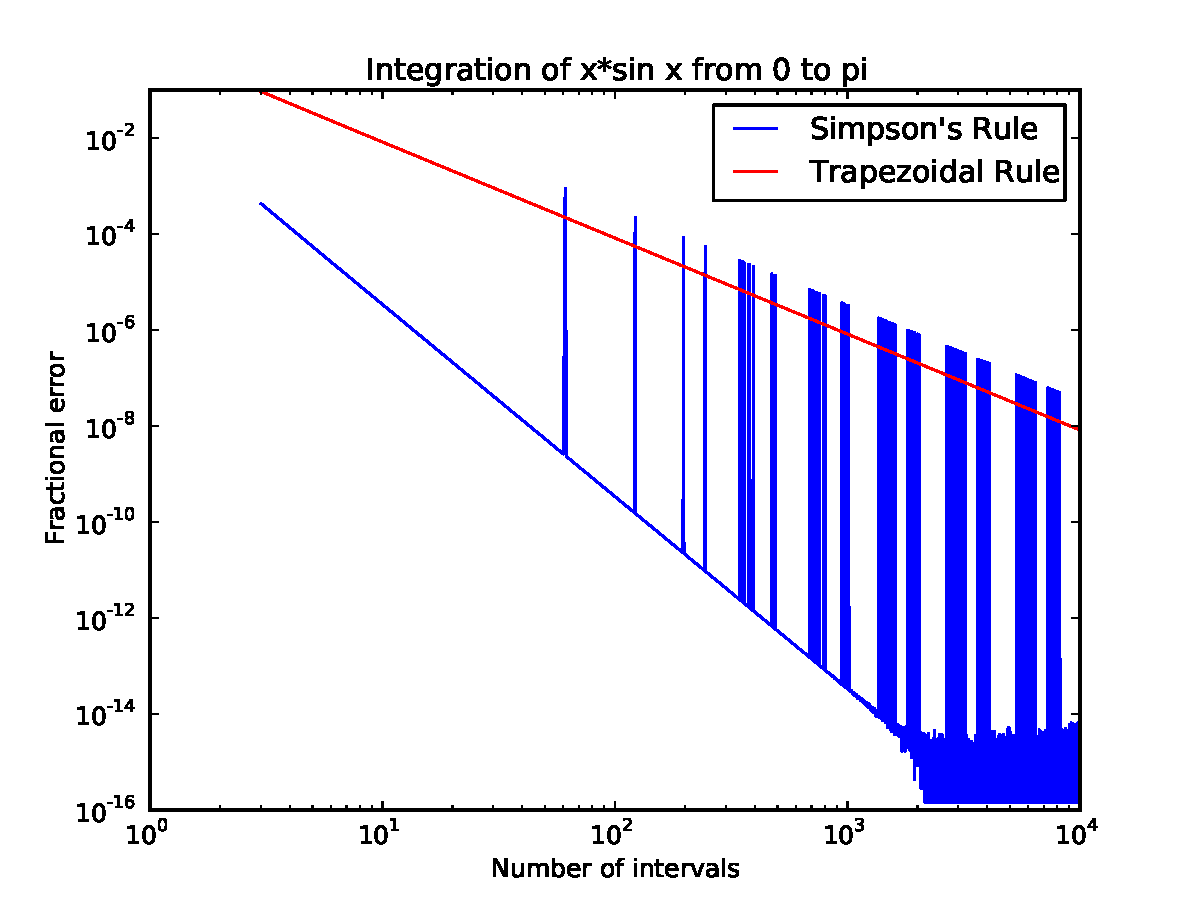
\includegraphics[width=\textwidth]{xsinx}
  \end{center}
  \caption{Fractional error on numerical integration of $x\sin(x)$ from 0 to $\pi$, using
	   the Trapezoid Rule and Simpson's Rule, for a range of step sizes.}
  \label{fig:xsinx}
\end{figure}

Figures \ref{fig:sinx} and \ref{fig:xsinx} show the fractional errors, (calculated answer - real answer)/(real answer),
of the integrations, which
decrease with increasing number of intervals $N$. $N = \pi/h$ for step size $h$.
Since the error on the Trapezoid Rule goes as $h^2$ or $N^{-2}$, the slope of
the error on the Trapezoid Rule is -2 on a log-log plot.  Similarly, Simpson's
Rule is $O(h^4)$, so the slope of the fractional error is -4 on the log-log plot.
The fractional error flattens out around $10^{-14}$, limited by floating-point
numerical precision.

There are a bunch of weird spikes in the error on Simpson's Rule, indicating that when
using Simpson's Rule, not all tiny step sizes are equal.  It's interesting to note that
the spikes follow the same slope as the Trapezoid Rule, rather than the slope of Simpson's Rule.

\section{Gaussian Quadrature}

We consider an environment where photons and electron-positron pairs are in equilibrium, so that the
electron/positron density is determined by the Fermi distribution.  
We assume a temperature of $k_BT = 20$ MeV, so that the electrons are highly relativistic.  The density
of electrons is determined by the integral:
\begin{equation}
	n_e = \frac{8\pi(k_BT)^3}{(2\pi\hbar c)^3} \int_0^\infty {\frac{x^2 dx}{e^x + 1}}
\end{equation}

\begin{figure}[h]
  \begin{center}
     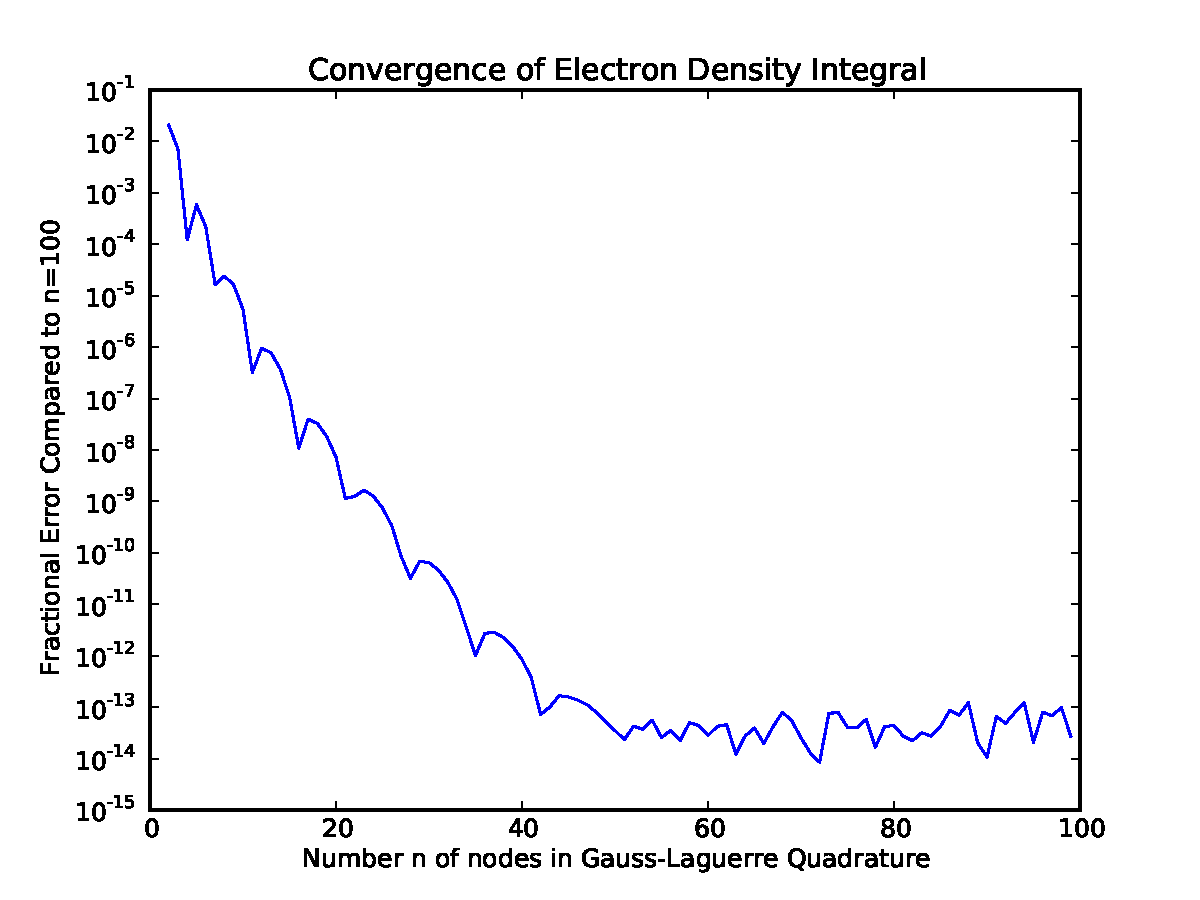
\includegraphics[width=\textwidth]{laguerre}
  \end{center}
  \caption{Fractional error on Gauss-Laguerre integration to obtain total electron density at $k_BT=20$ MeV,
	   for n nodes.}
  \label{fig:laguerre}
\end{figure}

\begin{figure}[h]
  \begin{center}
     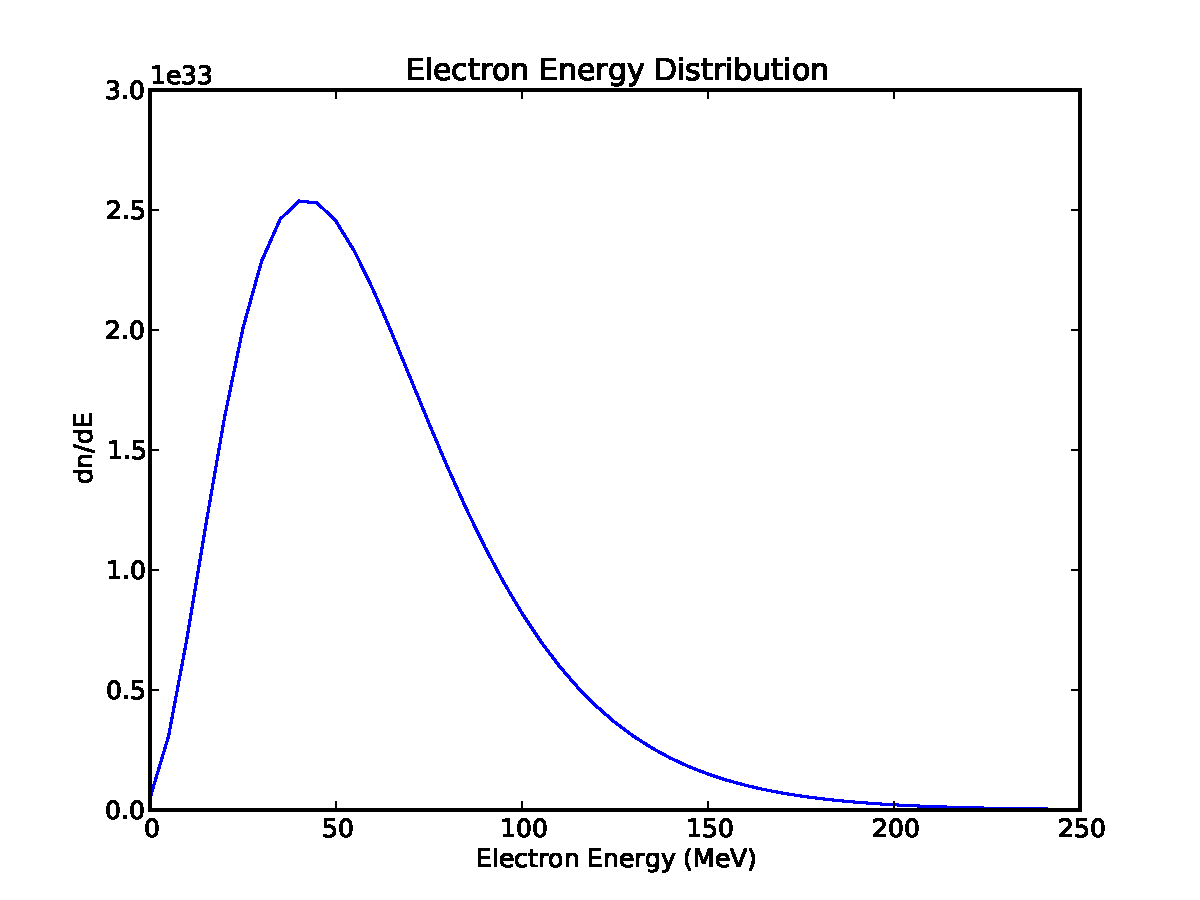
\includegraphics[width=\textwidth]{legendre}
  \end{center}
  \caption{Electron energy distribution, obtained by Gauss-Legendre integration over 5 MeV intervals.}
  \label{fig:legendre}
\end{figure}

I used Gauss-Laguerre integration, which is useful for integrals that are unbounded on one end, to solve this
integral, obtaining a total electron density of $1.902x10^{35}$ cm${^-3}$ for n=150 nodes.  Figure
\ref{fig:laguerre} shows the fractional error on this integral, calculated by considering the n=100 solution
to be the ``true'' solution.  The fractional error flattens off between $10^{-13}$ and $10^{-14}$ due to
floating-point rounding error.

Figure \ref{fig:legendre} shows the electron energy spectrum, $dn_e/dE$, from 0 to 250 MeV.  I used Gauss-Legendre
integration over intervals of 5 MeV to calculate the density of electrons in that energy range, and divided by the
interval width to get the derivative.  When I add up the derivative from 0 to 250 MeV and multiply by the interval width (effectively integrating), I obtain $n_e = 1.901x10^{35}$, consistent with the previous integration.

\end{document}